\documentclass[openany,a4paper,oneside,11pt]{article}

\usepackage{amsmath,amsfonts,amsthm,physics,braket,indentfirst}
\usepackage{float}

\usepackage[a4paper,
            left=3cm,
            right=3cm,
            top=3cm,
            bottom=3cm]{geometry}

\usepackage{lipsum}

\usepackage{graphicx}

\usepackage{hyperref}
\hypersetup{
	colorlinks=true,       	
	linkcolor=blue,          	
	citecolor=blue,        		
	urlcolor=blue}
\usepackage{url}

\newtheorem{alg}{Algorithm}
\newtheorem{exe}{Exercise}

\title{Numerical propagation in turbulent media}
\author{M. Gil de Oliveira}
\date{\today}

\begin{document}

\maketitle


\section{Propagation in free space}

Although we aim to study the propagation of light in turbulent media, it is important to first understand how light propagates in free space. This will provide us with a solid foundation for understanding the effects of turbulence on light propagation.

\subsection{The paraxial wave equation}

Our starting point will be the wave equation for the electric field, which is derived from Maxwell's equations. In free space, the wave equation can be expressed as
\begin{equation}
    \label{eq:wave equation}
    \nabla^2 E - \frac{1}{c^2} \partial_t^2 E = 0,
\end{equation}
where $E$ is the electric field, which we assumed to have a fixed polarization, $c$ is the speed of light in vacuum, and $\nabla^2$ is the Laplacian operator in three-dimensional space. 

A well known class of solutions are the plane waves $E(\mathbf{r}, t) = E_0 e^{i(\mathbf{k} \cdot \mathbf{r} - \omega t)}$ satisfies this equation, where $\mathbf{k}$ is the wave vector, $\omega$ is the frequency, and $E_0$ is a constant amplitude. The norm of the wave vector is related to the frequency $\omega$ by $ck = \omega$. These solutions have a well-defined direction of propagation defined by the wave vector $\mathbf{k}$, which we assume to be the $z$ direction, i.e., $\mathbf{k} = k \hat{\mathbf{z}}$.

Nonetheless, this class of solutions is nonphysical, as the electric field is not localized in space and contains an infinite amount of energy. A more physically relevant solution can be obtained by considering a field of the form
\begin{equation}
    E(\mathbf{r}, t) = u(\mathbf{r}) e^{i(kz - \omega t)},
\end{equation}
where $u(\mathbf{r})$ is a complex function describing an envelope that modulates the plane wave. By substituting this expression into the wave equation \eqref{eq:wave equation}, we obtain
\begin{equation}
    \nabla^2 u + 2ik \partial_z u= 0.
\end{equation}

\begin{figure}[]
    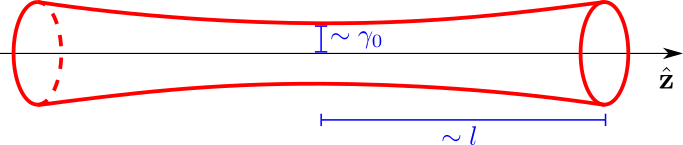
\includegraphics[scale=0.7]{feixe_paraxial.png}
    \centering
    \caption{Envelope of a paraxial beam.}
    \label{fig: paraxial beam}
\end{figure}

The typical envelope of a laser beam is shown in Fig. \ref{fig: paraxial beam}. The envelope $u(\mathbf{r})$ varies slowly along the $z$ direction. More precisely, the variation of $u$ in the $z$ is much smaller than the scale of variation defined by the wavenumber $k$. Therefore, we will assume that $\partial_z^2 u \ll k \partial_z u$, which allows us to neglect the second derivative with respect to $z$ in the wave equation. This leads us to the paraxial wave equation
\begin{equation}
\label{eq:paraxial}
    \nabla^2_T u + 2ik \partial_z u = 0,
\end{equation}
where $\nabla^2_T$ is the Laplacian operator restricted to the transverse plane, i.e., $\nabla^2_T = \partial_x^2 + \partial_y^2$.

\subsection{Solution of the paraxial wave equation}

The paraxial wave equation \eqref{eq:paraxial} is a partial differential equation that describes the propagation of light beams in the paraxial approximation. We want to find a solution for this equation, which will allow us to understand how light propagates in free space. In particular, we want to find a solution for the electric field envelope $u(x,y,z)$ given an initial condition $u(x,y,0)$ at $z=0$.

As it the equation is, the most straightforward way to solve it is to use the Fourier transform. Let us then define the Fourier transform of $u(x,y,z)$ as
\begin{equation}
\label{eq:fourier_transform}
    \tilde{u}(k_x, k_y,z) = \int_{\mathbb{R}^2} dx dy \ e^{-i(k_x x + k_y y)} u(x,y,z),
\end{equation}
which can be inverted as
\begin{equation}
\label{eq:inverse_fourier_transform}
    u(x,y,z) = \frac{1}{(2\pi)^2} \int_{\mathbb{R}^2} dk_x dk_y \ e^{i(k_x x + k_y y)} \tilde{u}(k_x, k_y,z).
\end{equation}
Substituting this expression into the paraxial wave equation \eqref{eq:paraxial}, we obtain
\begin{equation}
    \left( -k_x^2 - k_y^2 + 2ik \partial_z \right) \tilde{u}(k_x, k_y,z) = 0.
\end{equation}
This is a simple ordinary differential equation in $z$ for each fixed pair $(k_x, k_y)$. The solution can be written as
\begin{equation}
\label{eq:solution_paraxial_fourier}
    \tilde{u}(k_x, k_y,z) = \tilde{u}(k_x, k_y,0) e^{-i(k_x^2 + k_y^2)z/2k}.
\end{equation}

This provides a step-by-step algorithm for solving the paraxial wave equation:
\begin{alg}[Angular spectrum method]
\leavevmode
\begin{enumerate}
    \item Compute the Fourier transform $\tilde{u}(k_x, k_y,0)$ of the initial condition $u(x,y,0)$ using \eqref{eq:fourier_transform}.
    \item For each pair $(k_x, k_y)$, compute the solution $\tilde{u}(k_x, k_y,z)$ using the formula \eqref{eq:solution_paraxial_fourier}.
    \item Finally, compute the inverse Fourier transform to obtain the solution $u(x,y,z)$.
\end{enumerate}
\end{alg}

This is the angular spectrum method, which is a powerful technique for solving the paraxial wave equation. It allows us to compute the solution in the Fourier domain, where the equation becomes much simpler to solve. This is the basis for the method we will use to numerically simulate the propagation of light in turbulent media.

An equivalent way to express the solution of the paraxial equation, that is more simple from the analytical point of view, is obtained by substituting the expression \eqref{eq:solution_paraxial_fourier} into the inverse Fourier transform \eqref{eq:inverse_fourier_transform} and applying the convolution theorem. \footnote{This theorem states that the Fourier transform of convolution is the product of the Fourier transforms.} This leads to the following expression for the solution:
\begin{equation}
\label{eq:fresnel_diffraction}
    u(x,y,z) = \frac{k}{2\pi i z} \int_{\mathbb{R}^2} dx^\prime dy^\prime u(x^\prime,y^\prime,0) e^{ik\left[ (x-x^\prime)^2 + (y-y^\prime)^2 \right] / 2z}.
\end{equation}

This is the so-called Fresnel diffraction integral \cite{goodman2017introduction, schmidt2010numerical}.

\begin{exe}
    Apply the Fresnel diffraction integral to solve the paraxial wave equation for the initial condition
    \begin{equation}
        u(x,y,0) = e^{-(x^2+y^2)/w^2},
    \end{equation}
    where $w$ is a constant that defines the width of the beam (waist). 
\end{exe}

The Fresnel diffraction formula can be simplified when the distance $z$ is sufficiently large. In fact, assume that our initial condition $u(x,y,0)$ is mostly localized in a disk of radius $w$ around the origin, i.e., $u(x,y,0) \approx 0$ for $x^2+y^2 > w^2$. Then, when $z \gg kw^2/2$, the term $k[(x^\prime)^2 + (y^\prime)^2] / 2z$ in the exponent of \eqref{eq:fresnel_diffraction} does not contribute to the integral, and we can approximate the Fresnel diffraction integral as
\begin{equation}
    u(x,y,z) \approx \frac{k e^{ik\left( x^2 + y^2 \right) / 2z}}{2\pi i z} \int_{\mathbb{R}^2} dx^\prime dy^\prime u(x^\prime,y^\prime,0) e^{ik\left( xx^\prime + yy^\prime \right) / z}.
\end{equation}
This is known as the Fraunhofer diffraction integral, and it describes the far-field propagation of light. We can then see that, within the Fraunhofer approximation, the propagation of light can be understood as a Fourier transform of the initial condition $u(x,y,0)$, modulated by a quadratic phase factor that depends on the distance $z$.

\subsection{Analogy with quantum mechanics}

The paraxial wave equation \eqref{eq:paraxial} is analogous to the Schrödinger equation in quantum mechanics
\begin{equation}
    i \partial_t \psi(x, y, t) = -\frac{\hbar^2}{2m} \nabla^2 \psi(x, y, t),
\end{equation}
which describes the evolution of a free particle with wave function $\psi(x, y, t)$ in a two-dimensional space. The analogy is particularly useful because it allows us to use the same mathematical techniques to solve both equations. In fact, the angular spectrum method can be seen as a Fourier transform method for solving the Schrödinger equation, where the wave function $\psi$ plays the role of the electric field envelope $u$.

If we assume that our wave propagates through a medium with a space-dependent refractive index $n(x,y)$, the paraxial wave equation becomes may be approximated as
\begin{equation}
    \nabla^2_T u + 2ik \partial_z u + k^2(n^2 - 1) u = 0,
\end{equation}
which is analogous to the Schrödinger equation with a potential, i.e.,
\begin{equation}
    i \partial_t \psi(x, y, t) = \left( -\frac{\hbar^2}{2m} \nabla^2 + V(x,y) \right) \psi(x, y, t).
\end{equation}
This is what happens, for example, inside a waveguide, with the refractive index $n(x,y)$ being responsible for confining the light to a specific region of space, just like a potential well confines a quantum particle.

This analogy can also be extended to understand the imaging properties of lenses \cite{stoler1981operator}.

\subsection{Numerical solution}

Although the angular spectrum method provides a clear algorithm for solving the paraxial wave equation, it is often more practical to implement it numerically. Although it may seem straightforward, there are some subtleties that need to be considered. In this section, we will discuss the numerical implementation of the angular spectrum method and how to avoid common pitfalls. The discussion will be based on the notes \cite{fftderiv}, which provides a detailed explanation of how to calculate derivatives based on the (Discrete) Fourier Transform. To simplify the notation, we will assume a single transverse dimension, i.e., we will consider the paraxial wave equation in 1D. The extension to 2D is straightforward. 

First, we need to recognize that any numerical implementation must handle discrete and finite data. The most straightforward way to proceed would then to implement the integrals in \eqref{eq:fourier_transform} and \eqref{eq:inverse_fourier_transform} as discrete sums. However, approaches based on the Discrete Fourier Transform (DFT) are often more efficient. The DFT is analogous of Fourier series and transform, but applied to discrete and finite data. For 1D data, the DFT is defined as
\begin{equation}
    \tilde{u}_n = \sum_{m=0}^{N-1} u_m e^{-2\pi i mn/N},
\end{equation}
where $u_m$ is the $m$-th element of the discrete data, $\tilde{u}_n$ is the $n$-th element of the transformed data, and $N$ is the total number of elements in the data. The inverse DFT is given by
\begin{equation}
    u_m = \frac{1}{N} \sum_{n=0}^{N-1} \tilde{u}_n e^{2\pi i mn/N}.
\end{equation}

The advantage of the DFT is that it can be computed efficiently using the Fast Fourier Transform (FFT) algorithm \cite{cooley1965algorithm}, which has a time complexity of $O(N \log N)$, compared to the $O(N^2)$ time complexity of the naive implementation.

The idea is not to discretize $u(x,z)$, but rather to write an interpolation formula, i.e., we attempt to express $u(x,z)$ as
\begin{equation}
\label{eq:interpolation}
    u(x,z) = \sum_{n=0}^{N-1} \tilde{u}_n(z) e^{2\pi i n x/L},
\end{equation}
where $\tilde{u}_m(z)$ are the Fourier coefficients, $L$ is the length of the interval in which we are interested, and $N$ is the number of points in the interval. This is simply a finite Fourier series. If we have access to the values $u_m(z) = u(x_m,z)$, where $x_m = m \Delta x, \ m=0, \ldots N-1$ and $\Delta x = L / N$, we can use the DFT to compute the Fourier coefficients $\tilde{u}_m(z)$.

One important aspect of this interpolation should be mentioned: the function $u$ will have a period $L$, that is, $u(x+L,z) = u(x,z)$. This means that this approach allows us to solve the paraxial wave equation \eqref{eq:paraxial} under periodic boundary conditions. This is not strictly the physical situation, and if there is intensity in the boundaries, we will observe artifacts in the solution. However, this is a common situation in numerical simulations, and non-physical effects can be minimized by choosing a sufficiently large $L$. 

\section{Propagation in turbulent media}

\bibliographystyle{unsrt} 
\bibliography{refs}

\end{document}
